\begin{figure}[H]
	\centering
	\begin{subfigure}{0.49\textwidth}
	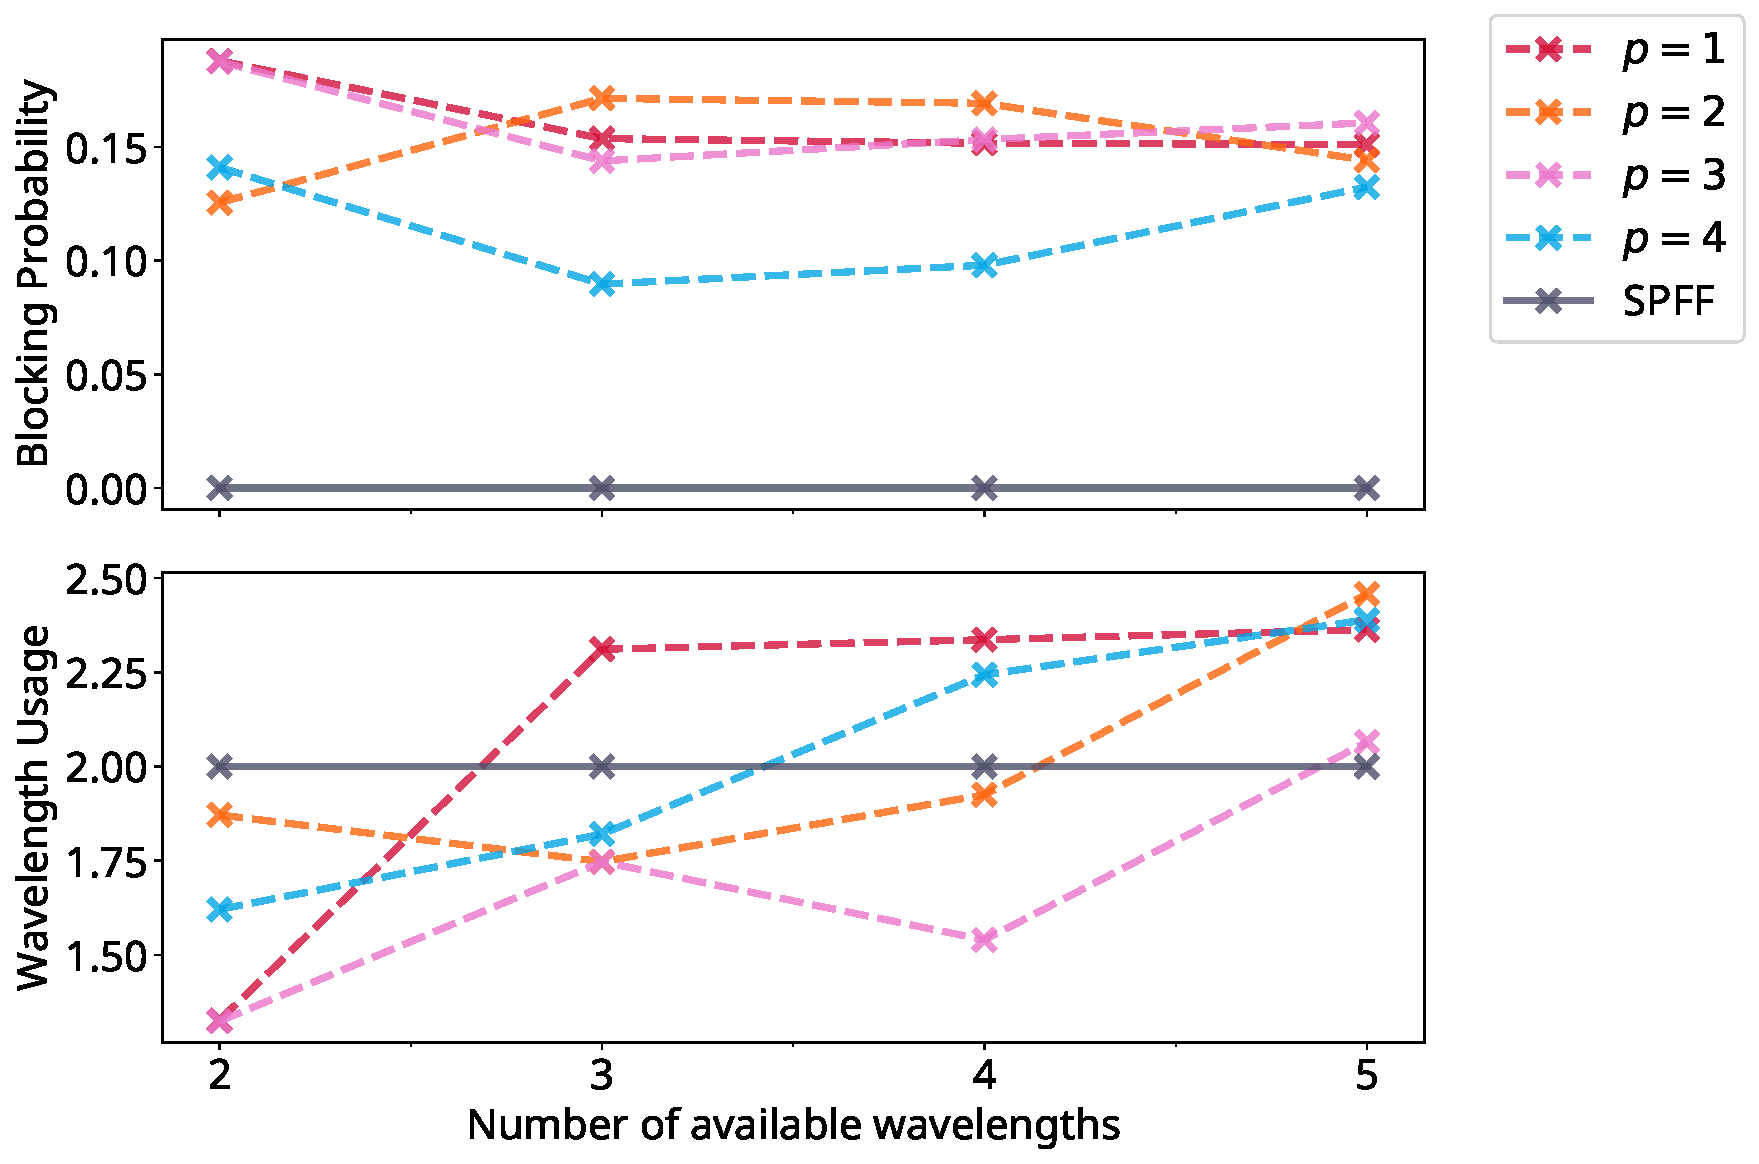
\includegraphics[width=\textwidth]{pictures/plots/n_wavelength/5-1-x-s.pdf}
	\caption{$N=5, \abs{P} = 1$, small topology}
	\end{subfigure}
	\begin{subfigure}{0.49\textwidth}
	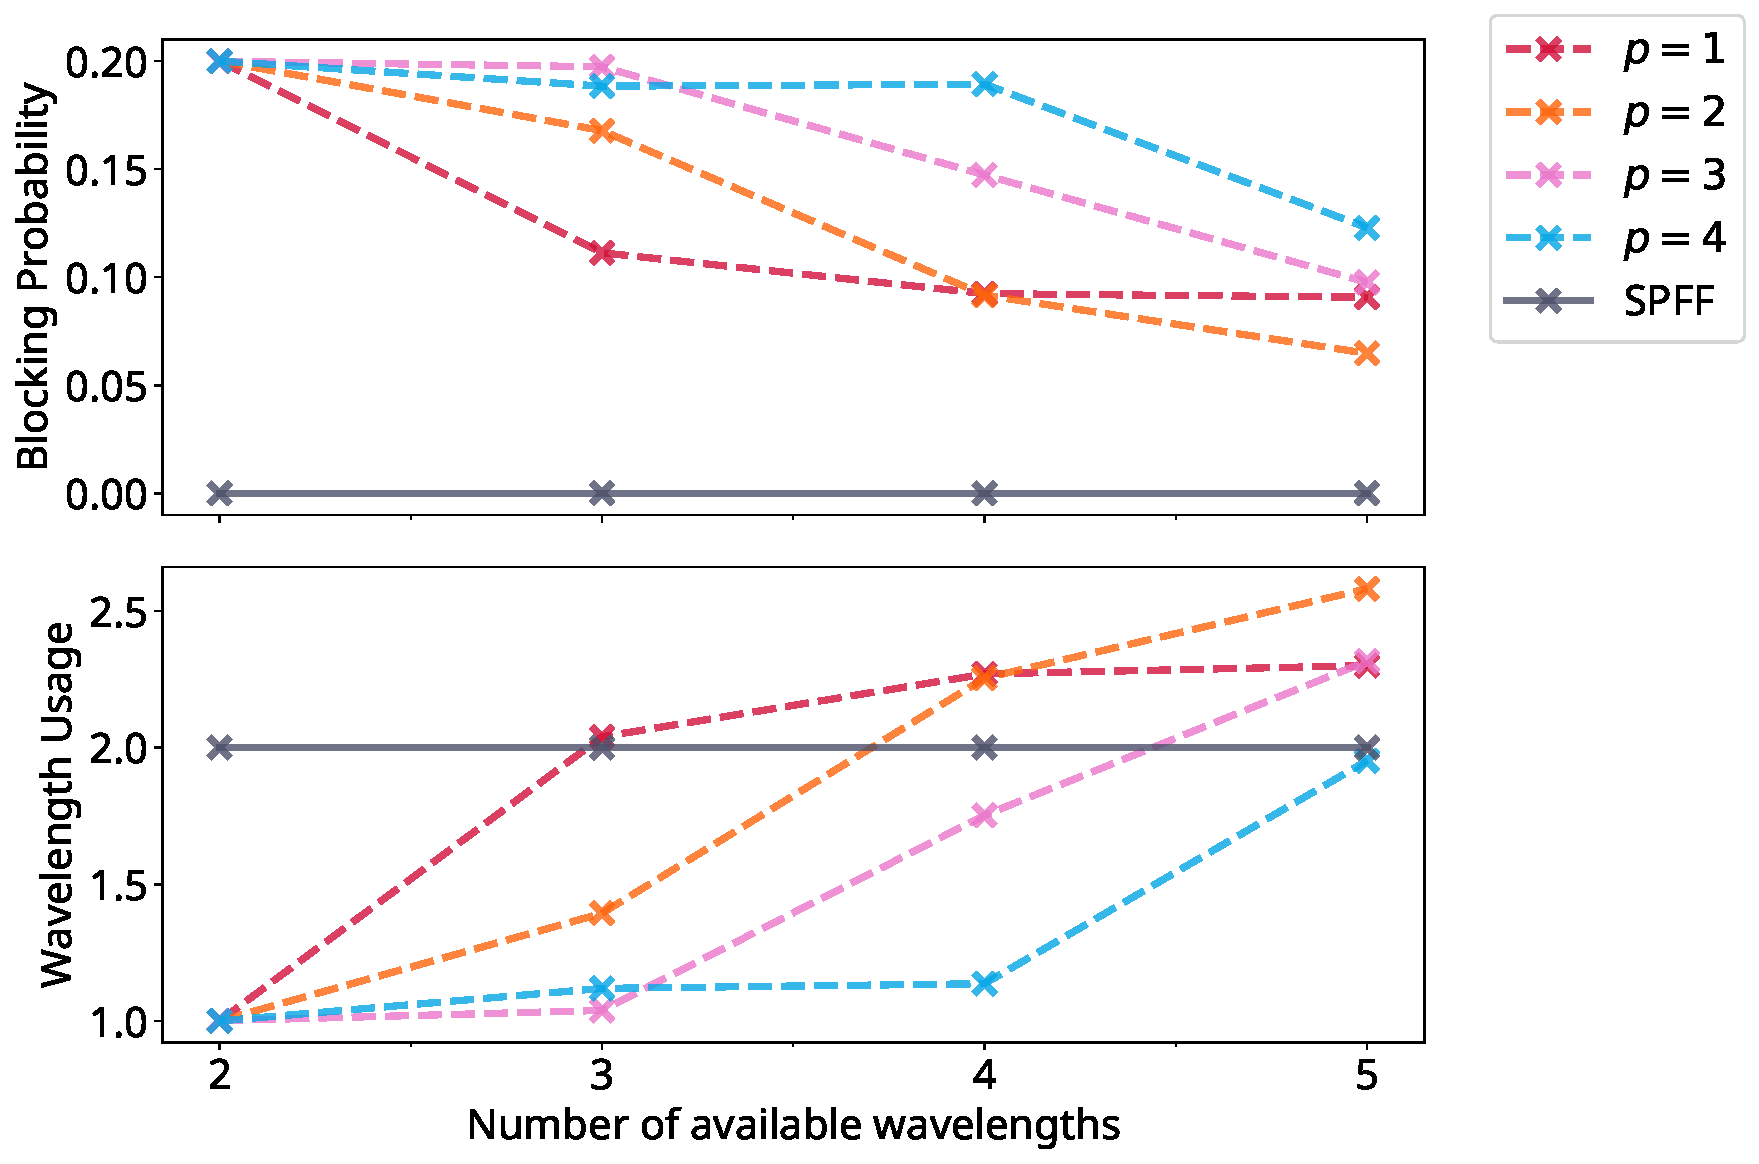
\includegraphics[width=\textwidth]{pictures/plots/n_wavelength/5-1-x-m.pdf}
	\caption{$N=5, \abs{P} = 1$, large topology}
	\end{subfigure}
\caption{The blocking probability and number of wavelength used.
\protect\reddashed represents $p=1$
\protect\peachdashed represents $p=2$
\protect\pinkdashed represents $p=3$
\protect\skydashed represents $p=4$
\protect\blackline represents SPFF
}
\label{fig:wavelengths}
\end{figure}
